\documentclass[11pt,a4paper]{article}
\usepackage[T1]{fontenc}
\usepackage[utf8]{inputenc}
\usepackage{lmodern,microtype}
\usepackage[margin=27mm,headheight=14pt]{geometry}
\usepackage{amsmath,amssymb,amsthm,mathtools}
\usepackage{booktabs,array,longtable}
\usepackage{enumitem}
\usepackage{xcolor,tikz,fancyhdr,hyperref}
\definecolor{ink}{HTML}{18364B}
\definecolor{accent}{HTML}{087F8C}
\hypersetup{colorlinks=true,linkcolor=ink,urlcolor=accent,citecolor=ink,
  pdftitle={Three triangle formulas in intuitionistic primitive recursive arithmetic},
  pdfauthor={Research prepared for Vladimir Reshetnikov}}
\pagestyle{fancy}
\fancyhf{}
\fancyhead[L]{\small\color{ink}Triangle formulas in intuitionistic PRA}
\fancyhead[R]{\small 14 November 2026}
\fancyfoot[C]{\thepage}
\setlength{\parskip}{4pt}
\setlength{\parindent}{1.1em}
\setlist{itemsep=3pt,topsep=5pt}
\newtheorem{theorem}{Theorem}[section]
\newtheorem{lemma}[theorem]{Lemma}
\newtheorem{proposition}[theorem]{Proposition}
\newtheorem{corollary}[theorem]{Corollary}
\theoremstyle{definition}
\newtheorem{definition}[theorem]{Definition}
\newtheorem{remark}[theorem]{Remark}
\newcommand{\ipra}{\mathsf{iPRA}}
\newcommand{\N}{\mathbb N}
\newcommand{\Q}{\mathbb Q}
\newcommand{\eps}{\varepsilon}
\newcommand{\abs}[1]{\left|#1\right|}
\newcommand{\norm}[1]{\left\lVert#1\right\rVert}
\newcommand{\ip}[2]{\left\langle#1,#2\right\rangle}
\newcommand{\rhoq}[2]{\rho_{#1}\!\left(#2\right)}
\newcommand{\code}[1]{\texttt{\small #1}}
\newcommand{\pr}{\mathrm{PR}}
\newcommand{\Apart}{\operatorname{Apart}}
\newcommand{\Reg}{\operatorname{Reg}}
\newcommand{\nn}{\operatorname{Nonneg}}
\newcommand{\Eq}{\operatorname{Eq}}
\numberwithin{equation}{section}

\begin{document}
\begin{center}
{\Large\bfseries\color{ink} Three triangle formulas in\\[3pt]
intuitionistic primitive recursive arithmetic}\\[9pt]
{\large Heron's formula, the law of sines, and the law of cosines}\\[7pt]
{\normalsize A complete mathematical argument, explicit finite error bounds,\\
and a concrete route to an internal Lean formalization}\\[9pt]
Prepared for Vladimir Reshetnikov\\
14 November 2026
\end{center}

\begin{abstract}
The three triangle formulas require very little analysis when angles are
represented by their geometric unit-ray coordinates. Their algebraic core is
the pair of polynomial identities
\[
 \norm{u-v}^{2}=\norm u^{2}+\norm v^{2}-2\ip uv,
 \qquad
 \norm u^{2}\norm v^{2}=\ip uv^{2}+\det(u,v)^{2}.
\]
We give complete proofs of the ordinary radical form of Heron's formula,
all three cosine laws, and the extended sine law including the circumradius.
Square roots are constructed by a bounded rational search. Division uses
explicit positive separation data. Quantitative rational theorems, with
fully specified precision schedules, express the results in first-order
intuitionistic primitive recursive arithmetic. A regular-name calculus then
gives a theorem schema for fixed primitive-recursive coordinate programs.
No completeness theorem, general excluded middle, choice, or induction on a
quantified Cauchy assertion is used.

The accompanying Lean files contain concrete algebraic proof scripts and
precise completion targets. They were not compiled in the delivery
environment, which has no Lean or Lake installation; the internal iPRA
formalization is an explicitly described remaining task. Independent exact
Python checks validate the fixed polynomial identities and numerical
certificates, and are distinguished from formal proof.
\end{abstract}

\section*{Results and scope at a glance}

For a triangle with side lengths \(a,b,c\), opposite geometric angles
\(A,B,C\), area \(\Delta\), semiperimeter \(s=(a+b+c)/2\), and circumradius
\(R\), the conclusions are
\begin{align*}
 \Delta&=\sqrt{s(s-a)(s-b)(s-c)},\\
 a^{2}&=b^{2}+c^{2}-2bc\cos A
       \quad\text{and its cyclic companions},\\
 \frac{a}{\sin A}&=\frac{b}{\sin B}
                 =\frac{c}{\sin C}=2R.
\end{align*}
Heron's formula includes degenerate triangles. The divided sine law and
circumcircle require a positive determinant-apartness witness. All three
formulas have a uniform finite arithmetic form. Assertions for general
primitive-recursively represented coordinates are first-order schemas,
not quantification over a sort of all real numbers.

\newpage
\begingroup
\small
\setlength{\parskip}{0pt}
\tableofcontents
\endgroup
\newpage

\section{The precise constructive setting}\label{sec:setting}

\subsection{The arithmetic theory}

We use first-order intuitionistic primitive recursive arithmetic
\(\ipra\): intuitionistic first-order logic with equality, a symbol for
each particular primitive-recursive construction, its defining equations,
\(Sx\ne0\), successor injectivity, and induction for quantifier-free
formulas with arbitrary numerical parameters. The function constructors
are zero, successor, projection, composition, and primitive recursion.
One may use the usual intuitionistic natural-deduction rules for
\(\bot,\wedge,\vee,\to,\forall,\exists\), with the ordinary eigenvariable
conditions. Quantifiers are allowed in theorems and hypotheses; their
presence does not enlarge the induction schema.

Order, finite tuples, signed integers, rationals, bounded searches, and
powers of two are definitional extensions by particular PR functions.
Decidable rational comparisons are legitimate. A proof by cases on such
a comparison is not an invocation of excluded middle for arbitrary
formulas. This is the first-order, quantifier-free-induction presentation
discussed in the foundational literature~\cite{moschovakis} and explicitly
implemented by the inspected ConciseIPRA project~\cite{pr-source}.

One possible coding uses even numbers for nonnegative integers and odd
numbers for negative integers:
\[
 \operatorname{code}(z)=
 \begin{cases}2z&z\ge0,\\-2z-1&z<0.\end{cases}
\]
A rational is a pair consisting of a signed numerator and a natural
denominator parameter \(d\), with actual denominator \(d+1\).
Unreduced fractions suffice. Rational equality and order are tested by
cross multiplication with positive denominators. For example,
\(\langle a,b\rangle=2^a(2b+1)-1\) is a PR pairing with PR projections:
the exponent of two in \(n+1\) is found by a search bounded by \(n+1\).
Thus all displayed rational statements are abbreviations for
first-order statements about natural numbers.

\subsection{What a real-looking theorem means here}

First-order \(\ipra\) has no variable ranging over all real numbers.
We give two precise levels of conclusion.

\begin{enumerate}
\item \textbf{Uniform finite theorems.} Rational coordinates, integer
bounds, a precision \(k\), and, where needed, a positive separation
witness are numerical inputs. Explicit PR computations satisfy explicit
rational error bounds. Section~\ref{sec:finite} states and proves these
theorems without any completed-real variables.
\item \textbf{A schema for fixed PR names.} Each coordinate is supplied
by one fixed PR rational approximation program, possibly with numerical
parameters, together with the regularity hypotheses below. The output
programs are again PR. The resulting equality assertions are ordinary
first-order formulas involving those particular function symbols.
Section~\ref{sec:names} gives the required arithmetic interpretation.
\end{enumerate}

This distinguishes a genuine internal arithmetic result from an ambient
Lean theorem over \(\mathbb R\). It also avoids a nonexistent total
primitive-recursive universal evaluator for all PR program codes.
Substitution of a fixed PR definition is allowed; universal unbounded
evaluation of an arbitrary PR-code input is not assumed.

\subsection{Constructive nondegeneracy}

For a represented scalar \(t\), the divided sine law uses supplied data
\(\abs t\ge\delta>0\), where a positive rational \(\delta\), or a smaller
dyadic \(2^{-d}\), is explicitly available. We call this
\emph{apartness}. A bare statement \(\neg(t=0)\) is not used to produce
such a witness. For nonzero rational \(t\), the witness is computable by
a bounded search; for named coordinates it is a stated hypothesis.

\section{A bounded construction of square roots}\label{sec:root}

Put \(\eps_k=2^{-k}\). If \(q=p/r\ge0\), where \(p\in\N\) and
\(r\ge1\), define
\[
 J=(p+1)2^k,\qquad
 j=\max\{i\le J:r i^2\le p\,2^{2k}\},\qquad
 \rhoq{k}{q}=\frac{j}{2^k}.
 \tag{2.1}\label{eq:root-program}
\]
The set contains zero, and the maximum is obtained by a bounded scan.
The routine is therefore PR. A zero-denominator input to an alternative
raw pair codec can be assigned the harmless output zero.

\begin{lemma}[The exact mesh bracket]\label{lem:mesh}
For every nonnegative rational \(q\) and \(k\in\N\),
\[
 \rhoq{k}{q}^{\,2}\le q
 <\bigl(\rhoq{k}{q}+\eps_k\bigr)^2.
 \tag{2.2}\label{eq:mesh}
\]
The assertion has a proof using quantifier-free induction.
\end{lemma}

\begin{proof}
For fixed \(p,r,k\), let \(S=2^k\), and let \(j_n\) be the last
successful index among \(0,\ldots,n\). Thus \(j_0=0\); at stage \(n+1\)
we replace \(j_n\) by \(n+1\) if \(r(n+1)^2\le pS^2\), and retain it
otherwise. Maintain the quantifier-free invariant
\[
 j_n\le n,\qquad rj_n^2\le pS^2,\qquad
 j_n<n\ \Longrightarrow\ pS^2<r(j_n+1)^2.
 \tag{2.3}\label{eq:scan-invariant}
\]
At zero this is immediate. If the new index passes, the first two
clauses hold and the third has false antecedent. If it fails, the old
third clause applies when \(j_n<n\); when \(j_n=n\), the failed test is
exactly the new third clause. The comparison \(j_n<n\) is decidable.
This proves the invariant by quantifier-free induction.

Since \(r\ge1\), \(S\ge1\), and \((p+1)^2>p\), we have
\[
 rJ^2\ge(p+1)^2S^2>pS^2.
\]
Consequently \(j_J<J\), by the invariant's lower bracket. Its third
clause gives the upper bracket at \(j_J+1\). Divide both inequalities
by the positive integer \(rS^2\).
\end{proof}

The formula already supplies arbitrarily narrow rational root intervals;
no root-existence theorem from analysis is needed. The implementation in
the archive uses a bounded binary search for efficiency and checks
the same two integer inequalities. The literal scan is included as a
reference implementation for small cases.

\begin{lemma}[Finite square comparison]\label{lem:square-compare}
For nonnegative rationals \(u,v\),
\[
 (u-v)^2\le\abs{u^2-v^2}.
 \tag{2.4}\label{eq:square-compare}
\]
In particular, \(\abs{u^2-v^2}\le\eta^2\) implies
\(\abs{u-v}\le\eta\) for rational \(\eta\ge0\).
If \(q,q'\ge0\), \(\abs{q-q'}\le\eta^2\), and \(r,r'\)
are lower mesh roots with mesh widths \(\alpha,\alpha'\), then
\[
 \abs{r-r'}\le\eta+\max(\alpha,\alpha').
 \tag{2.5}\label{eq:mesh-stability}
\]
\end{lemma}

\begin{proof}
Decide whether \(u\ge v\). In that case
\((u-v)^2\le(u-v)(u+v)=u^2-v^2\); the other case is symmetric.
Order comparison of nonnegative rational squares is equivalent to order
comparison of their bases, by factoring the difference of squares.
For the last assertion, if \(r\ge r'\), then
\[
 r^2\le q\le q'+\eta^2
 <(r'+\alpha')^2+\eta^2
 \le(r'+\alpha'+\eta)^2.
\]
Thus \(r-r'<\alpha'+\eta\). Reverse the roles in the other case.
Every comparison in this proof is between rationals.
\end{proof}

\section{A complete arithmetic interpretation of scalar notation}
\label{sec:names}

This section justifies the ordinary algebra used later. Readers interested
first in the geometric argument may turn to Section~\ref{sec:geometry};
the independently stated finite theorems in Section~\ref{sec:finite} also
make the internal arithmetic content explicit.

\subsection{Names, equality, and the tightening principle}

\begin{definition}
A bounded regular name \(x\) consists of a fixed PR rational function
\(n\mapsto x_n\) and a supplied natural bound \(M_x\ge1\), with
\[
 \abs{x_m-x_n}\le\eps_m+\eps_n,\qquad
 \abs{x_n}\le M_x\qquad(m,n\in\N).
 \tag{3.1}\label{eq:regular}
\]
Define
\setcounter{equation}{1}
\begin{align}
 x\sim y&\quad\Longleftrightarrow\quad
      \forall k\;\abs{x_k-y_k}\le2\eps_k,\label{eq:name-eq}\\
 x\ge0&\quad\Longleftrightarrow\quad
      \forall k\;x_k\ge-\eps_k,\label{eq:name-positive}\\
 \Apart_d(x)&\quad\Longleftrightarrow\quad
      \forall k\;\abs{x_k}\ge2^{-d}-\eps_k.\label{eq:name-apart}
\end{align}
Positive lower bounds use the corresponding signed version:
\(x_k\ge\delta-\eps_k\). Rational constants have constant names.
\end{definition}

These are first-order formulas for each fixed program, not new sorts.
Every regular name has a natural bound, for example a ceiling of
\(\abs{x_0}+2\); we retain it explicitly so precision schedules are
visible. The bounds used as subscripts below are always natural numbers.

\begin{lemma}[Rational tightening]\label{lem:tighten}
If rational \(q,r,C\), \(C\ge0\), satisfy
\(q\le r+C2^{-n}\) for every natural \(n\), then \(q\le r\).
The proof is intuitionistic and available in \(\ipra\).
\end{lemma}

\begin{proof}
Decide the rational comparison \(q\le r\). In the other case write
\(q-r=A/B\), \(A,B\ge1\), and \(C=c/d\), \(c\ge0,d\ge1\).
If \(c=0\) there is an immediate contradiction. Otherwise use the
explicit index \(n=Bc+1\). Quantifier-free induction proves
\(2^n\ge n+1>Bc\), whence
\[
 C2^{-n}<1/B\le A/B.
\]
The supplied inequality at this index is impossible. This is
case analysis on a decidable atom, not double-negation elimination
for an arbitrary proposition.
\end{proof}

In particular, \(\sim\) is an equivalence relation. To check the
only nontrivial part, suppose \(x\sim y\sim z\). For fixed \(k\)
and arbitrary \(n\), compare through \(x_n,y_n,z_n\) to get
\[
 \abs{x_k-z_k}\le2\eps_k+6\eps_n.
\]
Tightening gives the required bound. A further useful consequence is
\[
 x\sim y\quad\Longrightarrow\quad
 \abs{x_m-y_n}\le\eps_m+\eps_n.
 \tag{3.5}\label{eq:cross}
\]
Compare through \(x_j,y_j\), obtaining an additional \(4\eps_j\),
and tighten. Nonnegativity and any specified lower bound are invariant
under \(\sim\), by the same argument. In particular,
\(x\sim r\) for a rational constant \(r\) is equivalent to
\(\abs{x_k-r}\le\eps_k\) at every \(k\).

\subsection{Explicit arithmetic operations}

The following table defines all operations needed in the proof.
Each recipe is a PR function once its input programs and numerical
bounds or witnesses are fixed.

\begin{center}
\renewcommand{\arraystretch}{1.3}
\begin{tabular}{@{}p{25mm}p{104mm}@{}}
\toprule
Operation & Output at precision \(k\)\\
\midrule
Negation & \(-x_k\)\\
Absolute value & \(\abs{x_k}\)\\
Addition & \(x_{k+2}+y_{k+2}\)\\
Multiplication &
\(x_{k+M_x+M_y+2}\,y_{k+M_x+M_y+2}\)\\
Reciprocal &
With \(\Apart_d(x)\), put \(N=k+2d+4\).
Return \(1/x_N\) if \(\abs{x_N}\ge2^{-d-1}\), and \(0\) otherwise.\\
Nonnegative root &
For \(x\ge0\), return
\(\rhoq{k+2}{\max(0,x_{2k+6})}\).\\
\bottomrule
\end{tabular}
\end{center}

Negation and absolute value preserve regularity immediately. Addition
has regularity bound \((\eps_m+\eps_n)/2\) and magnitude bound
\(M_x+M_y\). For multiplication let \(h=M_x+M_y+2\). The identity
\(ab-a'b'=a(b-b')+b'(a-a')\) gives
\[
 \abs{x_{m+h}y_{m+h}-x_{n+h}y_{n+h}}
 \le(M_x+M_y)2^{-h}(\eps_m+\eps_n)
 \le\eps_m+\eps_n.
 \tag{3.6}
\]
Its magnitude bound is \(M_xM_y\). Positivity is preserved for
nonnegative inputs: if the sampled rational product is negative,
one factor is negative with magnitude at most the input error, and
the other has its supplied magnitude bound. The precision shift
makes the negative part at most \(\eps_k\).

For inversion, \(\eps_{k+2d+4}\le2^{-d}/16\), so
\(\abs{x_N}\ge15\cdot2^{-d}/16>2^{-d-1}\).
Thus the fallback branch is never taken under the hypothesis, the
output is bounded by \(2^{d+1}\), and
\[
 \abs{\frac1{x_{m+2d+4}}-\frac1{x_{n+2d+4}}}
 \le2^{2d+2}
   \bigl(\eps_{m+2d+4}+\eps_{n+2d+4}\bigr)
 =\frac14(\eps_m+\eps_n).
 \tag{3.7}\label{eq:inverse-regular}
\]
A nonnegative apart input gives a positive reciprocal. This is checked
at the sampled rational: a negative sample would have magnitude at
most its error and also magnitude greater than \(2^{-d-1}\), which is
impossible.

\subsection{Root regularity and correctness, including zero}

For clarity, general order on names is defined by
\(x\le y\) if the difference name \(y-x\) is nonnegative.
It has the useful equivalent form
\[
 x\le y\quad\Longleftrightarrow\quad
 \forall n\;x_n\le y_n+2\eps_n.
 \tag{3.7a}\label{eq:order-test}
\]
For the reverse implication, sample the right-hand bound at
\(n=k+2\), giving \((y-x)_k\ge-2\eps_{k+2}\ge-\eps_k\).
For the forward implication, compare \(x_k-y_k\) through the
sample at \(n+2\). Its upper bound is
\(2\eps_k+2\eps_{n+2}+\eps_n\); tighten in \(n\).
If one side is a constant rational \(\delta\), the same comparison
has only one varying name and sharpens to
\(x_k\ge\delta-\eps_k\) for \(\delta\le x\).

Write \(q_k=\max(0,x_{2k+6})\) and \(r_k=\rhoq{k+2}{q_k}\).
The positive-part function is rationally \(1\)-Lipschitz, and hence
\[
 \abs{q_m-q_n}\le2^{-2m-6}+2^{-2n-6}
 \le\left(\frac{\eps_m+\eps_n}{8}\right)^2.
\]
Apply Lemma~\ref{lem:square-compare} with meshes
\(\alpha_i=\eps_i/4\) to obtain
\[
 \abs{r_m-r_n}\le
 \max(\alpha_m,\alpha_n)+\frac{\eps_m+\eps_n}{8}
 \le\frac38(\eps_m+\eps_n).
 \tag{3.8}
\]
All \(r_k\) are nonnegative, and \(B=M_x+1\) is a natural magnitude
bound. The mesh bracket and \(x\ge0\) give
\[
 \abs{r_k^2-x_{2k+6}}
 \le2B\alpha_k+\alpha_k^2+\eps_{2k+6}
 \le(2B+2)\eps_k.
 \tag{3.9}\label{eq:root-square-error}
\]
The squared name \(r\cdot r\) samples \(r_N^2\) at \(N=k+2B+2\).
Consequently
\[
 \abs{(r\cdot r)_k-x_k}
 \le\eps_k+(2B+3)\eps_N\le2\eps_k.
\]
Thus \(r^2\sim x\). This constructs a nonnegative root without
dividing by a root or assuming its input is apart from zero.

\begin{lemma}[Uniqueness and comparison of nonnegative roots]
\label{lem:unique-root}
If nonnegative regular names \(u,v\) have \(u^2\sim v^2\), then
\(u\sim v\). More generally, \(u,v\ge0\) and \(u^2\le v^2\)
imply \(u\le v\); hence the constructed nonnegative square root
is monotone.
\end{lemma}

\begin{proof}
The uniqueness argument can be made entirely quantitative. Compare
\(u_N^2,v_N^2\) through arbitrarily finer samples of their squared
names, use~\eqref{eq:cross}, and tighten. This gives
\[
 \abs{u_N^2-v_N^2}\le2(M_u+M_v)\eps_N.
 \tag{3.10}
\]
Indeed changing \(u_N\) to \(u_m\) changes its square by at most
\(2M_u(\eps_N+\eps_m)\), with the analogous bound for \(v\);
the difference of the two sufficiently fine squared names tends to
zero with an explicit constant times \(\eps_m\).
Replace \(u_N,v_N\) by their positive parts \(U_N,V_N\).
Each replacement changes the value by at most \(\eps_N\) and the
square by at most \(\eps_N^2\). With
\(C=2(M_u+M_v+1)\), we obtain
\[
 \abs{U_N^2-V_N^2}\le C\eps_N.
\]
For a free precision \(r\), choose \(N=2r+C+1\); then
\(C\eps_N\le\eps_r^2\). Lemma~\ref{lem:square-compare}
gives \(\abs{U_N-V_N}\le\eps_r\).
For fixed \(k\), regularity now yields
\(\abs{u_k-v_k}\le2\eps_k+5\eps_r\).
Tighten in \(r\) and then generalize \(k\).

For monotonicity, use the same proof with the positive part of
\(U_N-V_N\) in place of its absolute value. If \(U_N\le V_N\)
there is nothing to prove. Otherwise
\((U_N-V_N)^2\le U_N^2-V_N^2\); the assumed order of the squared
names bounds the latter's positive part by a constant times
\(\eps_N\). The preceding precision choice and tightening prove
the order of the names. All case distinctions are rational.
\end{proof}

\subsection{Why the ordinary algebra is legitimate}

The operations respect \(\sim\), and their represented values are
independent of the supplied valid magnitude bounds or apartness
witnesses. Compare two outputs with a common arbitrarily fine input
stage and use~\eqref{eq:cross}, the product estimate (3.6), the
reciprocal estimate (3.7), and the root comparison lemma. For roots,
independence also follows from nonnegativity, square correctness,
and uniqueness.

Here is an explicit comparison bound for every ring identity
subsequently used. For each fixed expression \(E\), retain its
natural magnitude bound \(B_E\), using sums and products of bounds
at the corresponding nodes. Define a natural coefficient \(L(E)\) by
\[
 \begin{gathered}
 L(\text{constant})=0,\qquad L(\text{input})=1,\qquad
 L(-E)=L(E),\\
 L(E+F)=L(E)+L(F),\qquad
 L(EF)=B_E L(F)+B_F L(E).
 \end{gathered}
\]
Let \(E^{\mathrm{rat}}_n\) be the same rational expression with
every input sampled at the common index \(n\).
The addition and product difference estimates, node by node, give
\[
 \abs{E_k-E^{\mathrm{rat}}_n}
 \le L(E)(\eps_k+\eps_n).
\]
The internal shifts only reduce the input errors, so this bound
also applies to the prescribed oversampled operations.
If rational expressions \(E,F\) are identically equal, take
\(n=k\) to obtain
\(\abs{E_k-F_k}\le C\eps_k\), where
\(C=2(L(E)+L(F))\).
Comparing through their values at an arbitrary fine index \(j\)
gives \(2\eps_k+(C+2)\eps_j\). Tightening proves equality
of the names. Substituting equivalent inputs works the same way,
using~\eqref{eq:cross} at the input nodes.
The inverse law follows from the exact rational equality
\(x_N(1/x_N)=1\) and the same comparison.

This proves associativity, commutativity, distributivity, substitution,
and inversion or cancellation of apart factors. It also proves the
usual compatibility of nonnegative order with addition and
multiplication, by the rational inequalities already given.
Absolute values satisfy \(\abs{x}^2=x^2\), again from the exact
sampled identity.

We do not assert a decidable linear order on arbitrary names or a
total inverse for every merely unequal-to-zero name. All later
divisors have explicit apartness witnesses. Nor is induction applied
to a formula quantifying over all precisions. The only inductions so
far prove elementary natural arithmetic and the quantifier-free scan
invariant. A fixed finite expression requires only a finite
composition of the displayed lemmas.

\section{Coordinates, area, and geometric angles}\label{sec:geometry}

\subsection{The algebraic data}

Translate vertex \(A\) to the origin, and set
\[
 u=B-A=(x,y),\qquad v=C-A=(z,w).
\]
Write
\begin{align}
 U&=x^2+y^2,& V&=z^2+w^2,&
 W&=(x-z)^2+(y-w)^2,\label{eq:uvw}\\
 p&=xz+yw,& t&=xw-yz,& h&=\abs t.\label{eq:pt}
\end{align}
The opposite side lengths and area are
\[
 a=\sqrt W,\qquad b=\sqrt V,\qquad c=\sqrt U,\qquad
 \Delta=h/2.
 \tag{4.3}\label{eq:sides-area}
\]
The scalar constructions above give the meaning of each radical.
The determinant area is the ordinary base-times-height area: when
\(c>0\), the unit normal to \(u\) is \((-y/c,x/c)\), and the height
of \(v\) above that line is \(h/c\). Thus half base times height
is \(h/2\). The determinant formula also defines the continuous
zero-area extension to degenerate triples.

\begin{figure}[ht]
\centering
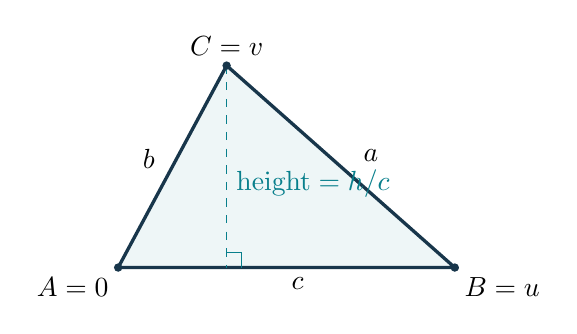
\begin{tikzpicture}[scale=0.95]
\coordinate (A) at (0,0);
\coordinate (B) at (4.5,0);
\coordinate (C) at (1.45,2.7);
\coordinate (H) at (1.45,0);
\fill[accent!7] (A)--(B)--(C)--cycle;
\draw[very thick,ink] (A)--(B)--(C)--cycle;
\draw[dashed,accent] (C)--(H);
\draw[accent] (1.45,0.2)--(1.65,0.2)--(1.65,0);
\fill[ink] (A) circle(1.6pt) (B) circle(1.6pt) (C) circle(1.6pt);
\node[below left] at (A) {\(A=0\)};
\node[below right] at (B) {\(B=u\)};
\node[above] at (C) {\(C=v\)};
\node[below] at (2.4,0) {\(c\)};
\node[left] at (0.62,1.45) {\(b\)};
\node[right] at (3.15,1.5) {\(a\)};
\node[right,accent] at (1.45,1.12) {\(\text{height}=h/c\)};
\end{tikzpicture}
\caption{An illustrative orientation. The proofs use signed dot products
and absolute determinants, and apply equally to obtuse and clockwise triangles.}
\end{figure}

\begin{lemma}[The finite algebraic nucleus]\label{lem:core}
\[
 W=U+V-2p,\qquad UV=p^2+t^2.
 \tag{4.4}\label{eq:core}
\]
\end{lemma}
\begin{proof}
Expanding the two coordinate differences gives the first identity.
For the second,
\[
 (xz+yw)^2+(xw-yz)^2
 =x^2z^2+x^2w^2+y^2z^2+y^2w^2
 =(x^2+y^2)(z^2+w^2).
\]
The mixed terms cancel. These are integer polynomial identities.
\end{proof}

\subsection{All necessary positive bounds}

Suppose the four coordinate magnitudes are at most a natural
\(M\ge1\), put \(Q=4M\), and suppose \(h\ge\delta>0\).
Then
\[
 0\le a,b,c\le Q,\qquad
 h\le bc,\quad h\le ca,\quad h\le ab.
 \tag{4.5}\label{eq:bounds}
\]
For example \(U,V\le2M^2\), \(W\le8M^2\), and \(UV\ge t^2\);
nonnegative square comparison gives the first incident-product
bound. The other two follow by applying the same identity at
vertices \(B,C\), whose determinants are \(-t,t\).
Consequently
\[
 a,b,c\ge\delta/Q,\qquad
 bc,ca,ab\ge\delta.
 \tag{4.6}\label{eq:side-lower}
\]
Every subsequent side division is therefore certified. A positive
rational bound can always be replaced by an explicitly smaller
dyadic: if the bound is \(A/B>0\) with \(A,B\ge1\), then
\(2^{-B}\le1/B\le A/B\). No unbounded search is needed.

\subsection{Angles as normalized unit-ray coordinates}

For nondegenerate triangles define the geometric angle values by
\setcounter{equation}{6}
\begin{align}
 \cos A&=\frac{p}{bc},&
 \sin A&=\frac{h}{bc},\label{eq:angle-a}\\
 \cos B&=\frac{U-p}{ca},&
 \sin B&=\frac{h}{ca},\label{eq:angle-b}\\
 \cos C&=\frac{V-p}{ab},&
 \sin C&=\frac{h}{ab}.\label{eq:angle-c}
\end{align}
This is the ordinary geometric definition of sine and cosine via
unit rays, rather than a definition by one of the laws to be proved.
Indeed the explicitly given orthogonal matrix
\[
 \begin{pmatrix}x/c&y/c\\-y/c&x/c\end{pmatrix}
\]
maps \(u/c\) to \((1,0)\) and \(v/b\) to
\((p/(bc),t/(bc))\). The nonoriented interior angle has the same
first coordinate and the nonnegative second coordinate.
At \(B\) the incident vectors are \(-u,v-u\); at \(C\) they are
\(-v,u-v\). Their dot products and determinant magnitudes are
exactly those in~\eqref{eq:angle-b}--\eqref{eq:angle-c}.
Dot products and absolute determinants are invariant under changes
of orthonormal coordinates, as follows by multiplying the matrices
and using \(Q^{\mathsf T}Q=I\).

The Gram identity proves
\[
 \cos^2 A+\sin^2 A=1
\]
and its cyclic companions. Moreover,
\[
 \sin A,\sin B,\sin C\ge\delta/Q^2>0.
 \tag{4.10}\label{eq:sin-lower}
\]
Thus these are upper-semicircle angle coordinates, including negative
cosines for obtuse angles. No decision whether an exact angle is
acute, right, or obtuse is made.

There is also an algebraic check of the angle-sum relation. Let
\(z_A=\cos A+i\sin A\), cyclically, with complex notation
abbreviating pairs and their multiplication. Since \(h^2=t^2\),
\[
 p(U-p)-h^2=U(p-V),\qquad hp+h(U-p)=hU,
\]
division by \(abc^2=abU\) gives
\[
 z_Az_B=-\overline{z_C},\qquad z_Az_Bz_C=-1.
 \tag{4.11}\label{eq:angle-sum}
\]
This is the usual supplementary-angle relation directly in
unit-circle coordinates.

Our angle variables denote geometric ray angles, not independently
constructed real radian measures. These are sufficient for the
geometric laws in the question. A separate identification with an
analytic library's \code{Real.sin} or \code{Real.cos} would be an
additional interface theorem, not an assumption hidden in this proof.

\section{The law of cosines}

\begin{theorem}\label{thm:cos}
For a nondegenerate triangle with the data above,
\begin{align*}
 a^2&=b^2+c^2-2bc\cos A,\\
 b^2&=c^2+a^2-2ca\cos B,\\
 c^2&=a^2+b^2-2ab\cos C.
\end{align*}
At an individual vertex only the two incident side lengths need
to be apart for that vertex's formula.
\end{theorem}

\begin{proof}
By definition \(bc\cos A=p\). Therefore the first identity
in~\eqref{eq:core} gives
\[
 a^2=W=U+V-2p=c^2+b^2-2bc\cos A.
\]
At \(B\), the squared length of the opposite edge is \(V\),
the two incident squared lengths are \(U,W\), and their dot
product is \(U-p\). Hence
\(V=U+W-2(U-p)\), which is the second formula.
At \(C\) the corresponding equation is
\(U=V+W-2(V-p)\), giving the third.
The proof is valid for either sign of each dot product.
\end{proof}

\section{The law of sines and the circumradius}

\begin{theorem}\label{thm:sine}
For a triangle with \(h\ge\delta>0\),
\[
 \frac{a}{\sin A}=\frac{b}{\sin B}
 =\frac{c}{\sin C}=\frac{abc}{h}=2R,
\]
where \(R\) is the radius of its explicitly constructed unique
circumcircle.
\end{theorem}

\begin{proof}
The bounds~\eqref{eq:side-lower} and~\eqref{eq:sin-lower}
justify every division. The first three equalities are immediate
from~\eqref{eq:angle-a}--\eqref{eq:angle-c}; for example
\(a/\sin A=a/(h/(bc))=abc/h\).

It remains to prove the circumradius assertion, rather than simply
give the common quotient a radius-like name. Define
\[
 N_x=Uw-Vy,\qquad N_y=Vx-Uz,\qquad
 O=\left(\frac{N_x}{2t},\frac{N_y}{2t}\right).
 \tag{6.1}\label{eq:center}
\]
The denominator is apart because \(\abs{2t}\ge2\delta\).
Finite expansion gives
\[
 xN_x+yN_y=Ut,\qquad zN_x+wN_y=Vt.
\]
Thus \(2\ip Ou=U\) and \(2\ip Ov=V\), and
\[
 \norm{O-u}^2=\norm O^2-2\ip Ou+U=\norm O^2,
 \quad
 \norm{O-v}^2=\norm O^2.
\]
Nonnegative-root uniqueness shows that \(O\) is equidistant from
the three vertices. If another point is equidistant, subtracting
its squared-distance equations yields the same two linear equations.
Eliminating one coordinate multiplies the other by \(t\);
cancellation of this apart determinant proves uniqueness.

The radius \(R=\sqrt{\norm O^2}\) now has its usual geometric
meaning. A second finite expansion gives
\begin{align*}
 N_x^2+N_y^2
 &=U^2V+V^2U-2UVp\\
 &=UV(U+V-2p)=UVW.
\end{align*}
Consequently \(4t^2R^2=UVW=a^2b^2c^2\).
The two nonnegative quantities \(2hR\) and \(abc\) have the same
square. By Lemma~\ref{lem:unique-root} they are equal.
Divide by the apart positive \(h\) to obtain \(2R=abc/h\).
\end{proof}

The cross-multiplied equations
\(b\sin A=a\sin B\) and \(c\sin A=a\sin C\)
also make sense for collinear triples with all side lengths apart.
The divided sine law and the circumcircle do not extend to those
triples; their sine values are zero.

\section{Heron's formula, including the radical}

\subsection{Triangle inequalities}

The Gram identity gives \(\abs p\le bc\), by nonnegative square
comparison. Therefore
\[
 a^2=b^2+c^2-2p\le b^2+c^2+2bc=(b+c)^2,
\]
so \(a\le b+c\). Repeating the argument gives the other two
triangle inequalities. No apartness is needed for these statements.

For a nondegenerate triangle they even have explicit strict
lower bounds. With the bounds of Section~\ref{sec:geometry},
\[
 (bc-p)(bc+p)=h^2\ge\delta^2,\qquad
 0\le bc-p\le2Q^2.
\]
Hence \(bc+p\ge\delta^2/(2Q^2)\). Since
\[
 (b+c-a)(a+b+c)=2(bc+p),\qquad a+b+c\le3Q,
\]
we obtain
\[
 b+c-a\ge\frac{\delta^2}{3Q^3}>0,
 \tag{7.1}\label{eq:strict-gap}
\]
and cyclically. This uses division only by positive rational
bounds, not by an unproved nonzero difference.

\subsection{The complete area proof}

\begin{theorem}[Heron's formula]\label{thm:heron}
For every represented coordinate triple, including a degenerate one,
put \(s=(a+b+c)/2\). Then
\[
 \Delta^2=s(s-a)(s-b)(s-c),\qquad
 \boxed{\ \Delta=\sqrt{s(s-a)(s-b)(s-c)}\ }.
\]
\end{theorem}

\begin{proof}
Using \(a^2=W,b^2=V,c^2=U\), the two identities
in~\eqref{eq:core} give
\[
 4t^2=4b^2c^2-(b^2+c^2-a^2)^2.
 \tag{7.2}
\]
Factor the right side by difference of squares:
\begin{align*}
 4b^2c^2-(b^2+c^2-a^2)^2
 &=\bigl((b+c)^2-a^2\bigr)
      \bigl(a^2-(b-c)^2\bigr)\\
 &=(a+b+c)(-a+b+c)(a-b+c)(a+b-c)\\
 &=16s(s-a)(s-b)(s-c).
\end{align*}
Since \(\Delta=h/2\) and \(h^2=t^2\),
\(16\Delta^2=4t^2\). Cancel the positive rational \(16\).
This proves the squared formula.

Each of the four semiperimeter factors is nonnegative by the
triangle inequalities; alternatively, nonnegativity of their product
already follows from the squared formula. The constructed
nonnegative square root of that product has the same square as the
nonnegative \(\Delta\). Lemma~\ref{lem:unique-root} identifies them.
Thus the argument proves the radical formula itself, and remains
valid when the area or a side is zero.
\end{proof}

\begin{remark}
The expanded identity
\[
 16\Delta^2=
 2a^2b^2+2b^2c^2+2c^2a^2-a^4-b^4-c^4
 \tag{7.3}\label{eq:heron-symmetric}
\]
is particularly convenient for finite numerical error bounds.
It is also a polynomial identity after the squared lengths are
substituted. The fixed algebraic identities have been checked by
independent exact coefficient expansion in the accompanying code.
\end{remark}

\section{Explicit finite theorems of arithmetic}\label{sec:finite}

We now eliminate the scalar-name notation from the conclusions.
All variables in this section denote rational codes or natural
numbers. All roots are finite computations \(\rho_n\) from
Section~\ref{sec:root}. Thus the universally closed results are
literal first-order \(\ipra\) theorems after expanding abbreviations.
The conservative precision bounds are chosen for simple proofs,
not for optimal running time.

\subsection{A finite Heron theorem with an explicit modulus}

Let \(x,y,z,w\in\Q\), let \(U,V,W,p,t\) be their exact rational
invariants, and let \(Q\ge1\) be a natural number with
\(U,V,W\le Q^2\). For example a coordinate bound \(M\ge1\)
gives \(Q=4M\). For a free precision \(k\), put
\begin{align*}
 n&=2k+4+3Q,&
 a_n&=\rhoq nW,& b_n&=\rhoq nV,& c_n&=\rhoq nU,\\
 s_n&=(a_n+b_n+c_n)/2,&
 P_n&=s_n(s_n-a_n)(s_n-b_n)(s_n-c_n),\\
 H_k&=\rhoq{k+1}{\max(P_n,0)},&
 \Delta&=\abs t/2.
\end{align*}

\begin{theorem}[Finite radical Heron]\label{thm:finite-heron}
With precisely these definitions,
\[
 \boxed{\ \abs{H_k-\Delta}\le2^{-k}\ }.
 \tag{8.1}\label{eq:finite-heron}
\]
No nondegeneracy or positive-area hypothesis is required.
\end{theorem}

\begin{proof}
Put \(\epsilon=2^{-n}\).
The mesh bracket gives \(0\le a_n,b_n,c_n\le Q\) and
\[
 0\le W-a_n^2,\ V-b_n^2,\ U-c_n^2
 \le(2Q+1)\epsilon\le3Q\epsilon.
 \tag{8.2}\label{eq:square-deficits}
\]
For example \(W<(a_n+\epsilon)^2\), and
\(\epsilon^2\le\epsilon\).

For any three rationals \(\alpha,\beta,\gamma\), the fixed
polynomial identity for the semiperimeter product reads
\[
 16P(\alpha,\beta,\gamma)
 =2(\alpha^2\beta^2+\beta^2\gamma^2+\gamma^2\alpha^2)
  -\alpha^4-\beta^4-\gamma^4.
 \]
Apply this at the three lower roots and compare with
\[
 4t^2=2(WV+VU+UW)-W^2-V^2-U^2.
 \]
Every squared side lies in \([0,Q^2]\) and changes by at most
\(3Q\epsilon\). A product of two such variables changes by
at most \(6Q^3\epsilon\), as does its square. There are three
product terms of coefficient \(2\) and three negative square
terms. Therefore
\[
 \abs{P_n-\Delta^2}
 \le\frac{54}{16}Q^3\epsilon
 \le4Q^3\epsilon
 \le2^{-2k-2}.
 \tag{8.3}\label{eq:finite-heron-square}
\]
The last inequality uses \(Q^3\le2^{3Q}\), a consequence of
the elementary quantifier-free bound \(Q\le2^Q\).

Clipping at zero cannot increase the distance to
\(\Delta^2\ge0\). Put \(\eta=2^{-k-1}\) and
\(q=\max(P_n,0)\); then \(\abs{q-\Delta^2}\le\eta^2\).
The mesh bracket for \(H_k\) has width \(\eta\).
If \(H_k\ge\Delta\), then
\(H_k^2\le q\le\Delta^2+\eta^2\), giving
\(H_k-\Delta\le\eta\) by square comparison.
If \(\Delta\ge H_k\), then
\[
 \Delta^2\le q+\eta^2
 <(H_k+\eta)^2+\eta^2
 \le(H_k+2\eta)^2,
 \]
giving \(\Delta-H_k\le2\eta\). These are decidable rational
cases. Thus \(\abs{H_k-\Delta}\le2\eta=2^{-k}\).
\end{proof}

The clipping concerns a finite approximant, whose side-rounding
errors may violate a triangle inequality near degeneracy. The exact
Heron radicand proved earlier is nonnegative. This numerical
convention does not alter the exact formula.

\subsection{Finite cosine and extended-sine theorems}

Assume now that \(x,y,z,w\) are rational, their magnitudes are at
most a natural \(M\ge1\), \(Q=4M\), and
\(h=\abs t\ge2^{-d}\) for a supplied natural \(d\).
For a free \(k\), define
\[
 n=2k+2d+5Q+8,\qquad
 a_n=\rhoq nW,\quad b_n=\rhoq nV,\quad c_n=\rhoq nU.
 \tag{8.4}\label{eq:trig-precision}
\]
Set
\begin{align*}
 C_A&=\frac p{b_nc_n},&
 C_B&=\frac{U-p}{c_na_n},&
 C_C&=\frac{V-p}{a_nb_n},\\
 S_A&=\frac h{b_nc_n},&
 S_B&=\frac h{c_na_n},&
 S_C&=\frac h{a_nb_n}.
\end{align*}
Compute the rational point \(O\) of~\eqref{eq:center}, and put
\[
 Q_R=O_x^2+O_y^2,\qquad
 R_k=\rhoq{k+2}{Q_R},\qquad K_n=\frac{a_nb_nc_n}{h}.
 \tag{8.5}
\]
The symbols \(C_A,S_A\) here are rational approximants, not exact
unit-circle coordinates. Their correctness as names follows from
the preceding construction and explicit denominator bounds.

\begin{theorem}[Finite trigonometric laws]\label{thm:finite-trig}
All displayed denominators are positive or apart as required, and
\begin{align*}
 \abs{a_n^2-b_n^2-c_n^2+2b_nc_n C_A}&\le2^{-k},\\
 \abs{b_n^2-c_n^2-a_n^2+2c_na_n C_B}&\le2^{-k},\\
 \abs{c_n^2-a_n^2-b_n^2+2a_nb_n C_C}&\le2^{-k},\\
 \frac{a_n}{S_A}
   =\frac{b_n}{S_B}
   =\frac{c_n}{S_C}&=K_n,\\
 \boxed{\ \abs{K_n-2R_k}\le2^{-k}\ }.&
\end{align*}
The equality of the three finite side-over-sine ratios is exact.
\end{theorem}

\begin{proof}
Write \(\delta=2^{-d}\) and \(\epsilon=2^{-n}\).
The cyclic Gram identities imply \(UV,UW,VW\ge\delta^2\).
Since \(U,V,W\le Q^2\), each of \(U,V,W\) is at least
\(\delta^2/Q^2\). For any lower root \(r\) of one of these
numbers, the mesh bracket and rational square comparison give
\[
 r+\epsilon>\delta/Q.
 \]
Our precision satisfies \(\epsilon\le\delta/(2Q)\);
indeed \(2Q\le2^{Q+1}\) and \(n\ge d+Q+1\).
Thus \(a_n,b_n,c_n\ge\delta/(2Q)>0\).
The \(S\)'s are positive and \(t\) is apart, so every division
is justified.

Let \(e_a=W-a_n^2\), \(e_b=V-b_n^2\),
\(e_c=U-c_n^2\). By~\eqref{eq:square-deficits}, each is in
\([0,3Q\epsilon]\). Since \(W-U-V+2p=0\),
\[
 a_n^2-b_n^2-c_n^2+2b_nc_n C_A
 =-e_a+e_b+e_c.
 \]
Its absolute value is at most \(9Q\epsilon\le2^{-k}\).
The cyclic computations are identical. The last inequality follows
from \(Q\le2^Q\) and the deliberately larger
precision~\eqref{eq:trig-precision}.

The sine-ratio equalities are direct rational cancellation.
For the radius comparison, the exact center identity gives
\(4h^2Q_R=UVW\). The three squared lower roots lie below
their targets, and a telescoping product difference gives
\[
 0\le UVW-a_n^2b_n^2c_n^2\le9Q^5\epsilon.
 \]
Consequently
\[
 0\le4Q_R-K_n^2
 \le9Q^5\,2^{2d-n}
 \le2^{-2k-4}.
 \tag{8.6}\label{eq:finite-radius-square}
\]
For the last step, \(Q^5\le2^{5Q}\), and
\(9/256\le1/16\).

Put \(\eta=2^{-k-2}\). The mesh bracket gives
\[
 R_k^2\le Q_R<(R_k+\eta)^2.
 \]
If \(K_n\ge2R_k\), then
\(K_n^2\le4Q_R<4(R_k+\eta)^2\), so
\(K_n-2R_k<2\eta\).
If \(2R_k\ge K_n\), then
\((2R_k)^2-K_n^2\le4Q_R-K_n^2\le\eta^2\),
so \(2R_k-K_n\le\eta\) by
Lemma~\ref{lem:square-compare}.
Thus \(\abs{K_n-2R_k}\le2\eta\le2^{-k}\).
No exact irrational quantity occurred in this proof.
\end{proof}

\subsection{The actual first-order sentence shape}

Let \(\mathbf q\) be a tuple of four rational codes. Each theorem
above becomes a universal closure of
\[
 \operatorname{Valid}(\mathbf q,M,d,k)
 \ \longrightarrow\
 \operatorname{Correct}(\mathbf q,M,d,k),
 \tag{8.7}
\]
with the unused inputs omitted for Heron. Both predicates are
quantifier-free after using PR characteristic functions for the
decidable comparisons. The bounded square-root scan is a function
symbol with the proved bracket, not an existential assertion about
an unbounded search.

Equivalently, define a total PR checker to output zero when the
input hypothesis is false or the displayed conclusions are true,
and one otherwise. The target is the universally closed equation
asserting that this specific checker is zero. Default outputs on
invalid inputs make all component programs total. The compiler
must preserve the particular definitions above; a different
constant-zero program would not satisfy the required correspondence.

Every step in the finite proofs is either a fixed polynomial
identity, rational arithmetic, a decidable case split, or an
instance of the root bracket and elementary power bounds.
Lemma~\ref{lem:mesh} supplies the only nontrivial algorithmic
invariant, and it is literally quantifier-free.

\section{General PR coordinates and side-length input}\label{sec:schema}

\subsection{The represented-coordinate theorem schema}

Fix four PR rational functions
\[
 f_x(\bar p,n),\quad f_y(\bar p,n),\quad
 f_z(\bar p,n),\quad f_w(\bar p,n),
\]
where \(\bar p\) is a finite tuple of numerical parameters. Let
\(\mathcal H(\bar p,\bar M)\) assert their four regularity and
magnitude-bound formulas~\eqref{eq:regular}.
Compose the explicit programs of Section~\ref{sec:names} to define
the sides, area, semiperimeter, and the two sides \(L_H,R_H\) of
Heron's formula. These are particular PR function definitions.
The exact arithmetic conclusion is
\[
 \ipra\ \vdash\
 \forall\bar p\,\forall\bar M\,
 \left(\mathcal H(\bar p,\bar M)\ \to\
       \forall k\,
       \abs{(L_H)_k-(R_H)_k}\le2^{1-k}\right).
 \tag{9.1}\label{eq:heron-schema}
\]
Here \(\abs{\cdot}\le2^{1-k}\) is rational-code notation.
There is a separate instance for each fixed tuple of PR definitions.
The displayed function letters are not quantified function variables.

The trigonometric schema adds \(\Apart_d(t)\) for the determinant
name constructed from these coordinates. Bounds (4.5)--(4.10)
produce explicit rational, hence dyadic, witnesses for every
denominator. The conclusion is the conjunction of the equality
formulas for the three cosine laws and the extended sine law.
Every side of every equation has an explicit regular-name program.

To prove these schemas inside \(\ipra\), assume the first-order
hypotheses, prove the pointwise operation lemmas of
Section~\ref{sec:names}, and perform the finite algebraic proofs of
Sections~4--7. Instantiating a naming hypothesis at a computed
index is ordinary universal elimination. The rational tightening
lemma is applied to fixed rational outputs; its proof chooses an
explicit index. Universal introduction then closes the free
precision variable. This gives the asserted derivation without
induction on \(\mathcal H\) or on a universally quantified
convergence assertion.

All results apply in particular to arbitrary rational-coordinate
triangles, and to irrational coordinates produced by the square-root
and arithmetic routines. The external interpretation in usual real
geometry agrees with these names because their moduli force unique
values; completeness of the classical real numbers is useful for
that external interpretation, but is not a premise of the internal
proof. A theorem literally quantifying over every real-valued
sequence belongs to a richer language; it is not being silently
identified with~\eqref{eq:heron-schema}.

\subsection{Constructing a triangle from three specified sides}

The coordinate presentation does not restrict the result to
triangles whose vertices are rational. Suppose represented positive
side lengths \(a,b,c\) are given, with positive lower-bound witnesses
for them and for all three triangle gaps. Put
\[
 A=(0,0),\qquad B=(c,0),\qquad
 r=\frac{b^2+c^2-a^2}{2c},\qquad
 C=\bigl(r,\sqrt{b^2-r^2}\bigr).
 \tag{9.2}\label{eq:side-construction}
\]
The radicand is positive by the independent polynomial identity
\[
 b^2-r^2=
 \frac{(a+b+c)(-a+b+c)(a-b+c)(a+b-c)}{4c^2}.
 \tag{9.3}
\]
This identity is simply difference-of-squares factorization; using
it here is not an appeal to the area conclusion of Heron's formula.
If the four numerator factors have positive rational lower
bounds \(f_1,\ldots,f_4\), and \(c\le C_0\), the radicand is at
least \(q_0=f_1f_2f_3f_4/(4C_0^2)>0\).
Its root has lower bound \(\min(q_0,1)\), since a nonnegative
number whose square is at least \(q_0\) is at least this quantity.
Multiplying by a lower bound for \(c\) supplies determinant apartness.

The distances satisfy
\[
 \norm{B-A}=c,\qquad
 \norm{C-A}^2=r^2+(b^2-r^2)=b^2,
\]
and
\[
 \norm{C-B}^2=(r-c)^2+(b^2-r^2)
 =b^2+c^2-2cr=a^2.
\]
Nonnegative-root uniqueness gives the desired side lengths.
This is a PR construction on the supplied names and witnesses.
For example \(a=b=c=1\) gives
\(B=(1,0)\), \(C=(1/2,\sqrt3/2)\),
\(\Delta=\sqrt3/4\), \(\cos A=1/2\),
\(\sin A=\sqrt3/2\), and \(R=1/\sqrt3\).
Thus even the elementary equilateral example is fully covered.

\section{Audit of the strength used}\label{sec:audit}

There are three distinct kinds of induction in a complete
arithmetization of this argument.

\begin{enumerate}
\item \textbf{Elementary natural arithmetic and coding.}
Addition, multiplication, comparison, pairing, quotient and
remainder with bounded algorithms, and powers of two have
quantifier-free accumulator invariants. Signed and rational
operations are fixed compositions of these. Denominators can be
left unreduced, so a greatest-common-divisor algorithm is optional.
\item \textbf{The bounded root scan.}
The invariant~\eqref{eq:scan-invariant} is a conjunction of
decidable comparisons and an implication between such comparisons.
Replace the comparisons by their PR characteristic equations if
an equality-only language is desired. No bounded quantifier is
being treated as syntactically quantifier-free without translation.
\item \textbf{Elementary size estimates.}
The estimates \(n+1\le2^n\) and \(Q^j\le2^{jQ}\) for the fixed
exponents \(j=3,5\) use ordinary quantifier-free induction and
finite multiplication. All precision schedules are explicit terms.
\end{enumerate}

The geometric identities themselves are fixed polynomial expansions.
Their proofs require only finitely many instances of ring laws.
The representation lemmas take arbitrary indices, instantiate
their hypotheses at finitely many computed indices, and prove
rational inequalities. Neither universal Cauchy properties nor
the final universal statements serve as induction formulas.

No use is made of the intermediate value theorem, compactness,
trigonometric power series, an analytic definition of \(\pi\),
choice, Markov's principle, or real trichotomy. The required
nonnegative-root uniqueness remains valid at zero; it was proved
without dividing by the sum of two roots. Every cancellation in
the divided geometric formulas has an explicit positive witness.

The argument is not a reduction to a consistency theorem for a
stronger system. The Busy Beaver and Diophantine consistency
developments mentioned in the question are useful possible sources
of arithmetic infrastructure, but none of their consistency
conclusions is required here.

\section{The Lean route and the inspected ProveIt sources}
\label{sec:lean}

\subsection{Source snapshot and existing results}

The repository inspection used the fixed ProveIt commit
\begin{center}
\code{38cafaa5be7f4602567440bcebc754abdbacefc9}.
\end{center}
Its toolchain and Mathlib requirement are version \code{v4.32.0}.
The source manifest in the archive records the pinned URLs and
the exact modules relevant to this proof.

There is already closely related geometry in the repository's
\code{Geometry.lean} module~\cite{geometry-source}, under
\begin{center}\small
\path{Algebra/SurrealNumbers/Surreal/Algebra/}.
\end{center}
It contains
\begin{itemize}
\item \code{Surreal.Complexify.normSq\_sub};
\item \code{Surreal.Complexify.dot\_sq\_add\_cross\_sq};
\item \code{Surreal.Complexify.heron\_factorization};
\item \code{Surreal.Complexify.heron}.
\end{itemize}
The surreal triangle modules also contain actual cosine and sine
laws~\cite{triangle-source}. The relevant declarations are:
\begin{center}
\begin{tabular}{ll}
\code{Triangle.cosine\_law} & \code{Triangle.sin\_angleA}\\
\code{Triangle.sine\_law} & \code{Triangle.sine\_law\_cyclic}
\end{tabular}
\end{center}
These support the choice of finite algebra, but their ambient
ordered-field, square-root, and surreal constructions do not by
themselves establish a derivation in \(\ipra\).

The appropriate small arithmetic foundation is in the directory
\begin{center}\small
\path{Logic/PrimitiveRecursiveArithmetic/ConciseIPRA/Lean/ConciseIPRA}.
\end{center}
The namespace is \code{LeanProofs.ConciseIPRA}. In particular:

\begin{center}
\renewcommand{\arraystretch}{1.15}
\begin{tabular}{@{}p{50mm}p{81mm}@{}}
\toprule
Module & Relevant actual declarations\\
\midrule
\code{Syntax.lean} & \code{Fm}, scoped terms, substitution, \code{Fm.QF}\\
\code{Deduction.lean} & \code{Prf Ax} for intuitionistic derivations\\
\code{PR.lean} & \code{PR}, \code{PTm}, \code{PRAAx},
\code{PRA.qfInd}, the PR defining-equation rules\\
\code{BiInterpretation.lean} & \code{pra\_iff\_teq},
transferring already constructed derivations\\
\code{NativeBiInterpretation.lean} & \code{NFm.ofPRA},
\code{pra\_iff\_native}\\
\bottomrule
\end{tabular}
\end{center}

The inspected \code{TeqArith.lean} also connects addition on its
term quotient to object derivability. We do not assume that a
complete internal ring-reflection facility is already available.
The direct replay route below works without such a facility.

\subsection{Delivered Lean artifacts and their exact status}

\begin{center}
\renewcommand{\arraystretch}{1.15}
\begin{tabular}{@{}p{43mm}p{88mm}@{}}
\toprule
File & Content and status\\
\midrule
\code{FiniteAlgebra.lean} &
Concrete \code{ring} scripts over a commutative ring: cosine, Gram,
Heron, circumcenter, and angle-pair numerator identities.
\textbf{Uncompiled}.\\
\code{RationalAlgebra.lean} &
Concrete rational denominator and square-comparison scripts.
\textbf{Uncompiled}.\\
\code{DyadicSpec.lean} &
Total bounded scan definitions and exact root-correctness
propositions. Their correctness proofs are specified work,
not completed theorems. \textbf{Uncompiled}.\\
\code{FiniteTargets.lean} &
Fully expanded proposition specifications for both quantitative
theorems of Section~8. Their proofs remain to be implemented.
\textbf{Uncompiled}.\\
\code{ObjectTargets.lean} &
Actual ConciseIPRA formula shape and conditional native transport.
The triangle-checker PR codes and their internal derivations
remain to be constructed. \textbf{Uncompiled}.\\
\code{OUTLINE.md} &
Detailed implementation order, API references, proof invariants,
and commands for a configured checkout.\\
\bottomrule
\end{tabular}
\end{center}

There was no Lean or Lake executable in the delivery environment.
No Lean-build success is claimed. The files contain no
\code{sorry}-based completion claims or added axioms, but the
absence of such placeholders is not a substitute for elaboration.
The complete human argument and the exact executed Python checks
are the completed deliverable layers available here.

\subsection{A concrete completion plan}

\begin{enumerate}
\item \textbf{Check the external polynomial kernel.}
In the pinned, configured ProveIt checkout, elaborate
\code{FiniteAlgebra.lean} and \code{RationalAlgebra.lean}.
The main generic statements are exactly
\[
 W=U+V-2p,\quad UV=p^2+t^2,\quad
 N_x^2+N_y^2=UVW,
\]
and the two Heron factorizations. The supplied proofs expose
coordinates directly and use \code{ring}.

\item \textbf{Construct the actual PR programs.}
Encode the arithmetic functions, rational codec, scan, and the
specific finite checker of each theorem as \code{PR} syntax trees.
Use the existing projection, composition, zero-recursion, and
successor-recursion rules to derive their defining equations.
Prove the required natural arithmetic and rational laws inside
\code{Prf PRAAx}. Prove that these syntax trees correspond to the
particular algorithms in Sections~2 and~8, including invalid-input
defaults.

\item \textbf{Replay the fixed algebra internally.}
Either write the few expansion derivations explicitly, or build a
derivation-producing polynomial normalizer with an internally
proved soundness lemma. An external invocation of \code{ring},
or a Python checker that returns true, does not automatically
produce the needed object proof. Direct replay is sufficient for
these fixed identities and avoids a large reflection development.

\item \textbf{Prove the exact scan bracket.}
Use \code{PRA.qfInd} on~\eqref{eq:scan-invariant}. Prove the
endpoint bound and derive the rational bracket. This discharges
the explicitly named \code{RootCorrectness} target after coding.
The upper-bracket argument has been given in full and has no
maximality quantifier hidden inside its induction formula.

\item \textbf{Formalize the finite residual estimates.}
Replay~\eqref{eq:square-deficits},
\eqref{eq:finite-heron-square}, and
\eqref{eq:finite-radius-square} by rational arithmetic.
Build internal proofs of the two finite theorem checkers being
zero. These yield the uniform rational-input endpoints before a
general named-scalar library is built.

\item \textbf{Add the regular-name schema.}
Implement the fixed program transformations, the equality and
order formulas, rational tightening, operation regularity, inverse
correctness, and root uniqueness. At each step the numerical
precision is a free variable; close it universally only after
the pointwise proof. Compose these lemmas to obtain
\eqref{eq:heron-schema} and the trigonometric schema.

\item \textbf{Transport only completed internal derivations.}
The required endpoint has the actual form
\[
 \code{Prf PRAAx [] (closeAll arity (checkerFormula checkCode))}.
 \]
The \code{checkCode} here must be the just-constructed code for
the specified checker. After this derivation exists,
\code{pra\_iff\_native} transports it to the native scalar
presentation. No step identifies an arbitrary Lean proof with
an object-theory proof.
\end{enumerate}

These are finite implementation obligations with concrete invariants
and statements, not an appeal to a missing analytic theorem.
The remaining work is substantial formal proof engineering:
the supplied scripts do not claim that it has already been done.

\section{Examples, exact checks, and reproducibility}
\label{sec:validation}

\subsection{Three illustrative triangles}

For \(u=(3,0)\), \(v=(0,4)\), we have
\[
 (U,V,W,p,t)=(9,16,25,0,12),\qquad
 (a,b,c,\Delta)=(5,4,3,6).
\]
Thus \(s=6\), Heron's radicand is \(6\cdot1\cdot2\cdot3=36\),
and the sine values are \(1,4/5,3/5\). Each side-over-sine
ratio is \(5\). The constructed center is \((3/2,2)\),
whose radius is \(5/2\).

For the obtuse example \(u=(2,0)\), \(v=(-1,1)\),
\[
 (U,V,W,p,t)=(4,2,10,-2,2).
\]
Here \(a=\sqrt{10}\), \(b=\sqrt2\), \(c=2\), and
\(\cos A=-1/\sqrt2\), \(\sin A=1/\sqrt2\).
The cosine law gives \(10=2+4+4\).
The center is \((1,2)\), so \(R=\sqrt5\); the common sine
ratio is \(2\sqrt5\). This explicitly tests the obtuse sign.

For \(u=(1,2)\), \(v=(2,4)\), the determinant and area vanish.
The side lengths satisfy an equality in the triangle inequality,
and Heron's radicand is zero. The finite Heron theorem still
applies at every precision. The divided sine law is not asserted.

\subsection{Executed verification}

The standard-library Python code uses integers and
\code{fractions.Fraction}; no floating-point computation is involved.
The delivered verification run passed:
\begin{center}
\begin{tabular}{@{}lr@{}}
\toprule
Exact check & Count\\
\midrule
Fixed integer-polynomial identities & 15\\
Rational root-bracket instances & 3696\\
Binary-root versus literal-scan comparisons & 140\\
Finite radical-Heron instances & 144\\
Finite cosine and extended-sine instances & 132\\
\bottomrule
\end{tabular}
\end{center}

The geometry cases include clockwise and obtuse triangles,
ordinary rational coordinates, a determinant of \(2^{-25}\),
collinear triples, coincident vertices, and the zero triple.
The numerical checks test precisions \(k=0,5,12\).
Each root computation checks its integer lower and upper bracket;
the geometry checks also verify the claimed rational residual
bounds. The polynomial checker is a separate small coefficient
normalizer with no computer-algebra-system dependency.

These computations are evidence against implementation and
constant errors. They are neither the mathematical proof for all
inputs nor a formally verified checker. The universal proofs are
the arguments above; the missing Lean status is recorded
separately in the archive.

\subsection{Reproducing the archive}

From the extracted \code{triangle\_ipra} directory, run:
\begin{verbatim}
python3 python/verify.py
pdflatex -output-format=pdf -halt-on-error triangle_formulas_ipra.tex
pdflatex -output-format=pdf -halt-on-error triangle_formulas_ipra.tex
\end{verbatim}
The first command writes \code{verification/results.json}.
The supplied \code{build.sh} runs the same sequence and stores
build logs under \code{verification}. Python 3.12.14 was used
for the recorded checks. The PDF was compiled from this
LaTeX source and inspected visually.

For Lean, follow \code{lean/OUTLINE.md} in a configured checkout
of the pinned ProveIt revision. The version pin alone does not
install Lean, retrieve Mathlib, or complete the internal proofs.

\begin{thebibliography}{9}

\bibitem{moschovakis}
Joan Rand Moschovakis.
\emph{Now Under Construction: Intuitionistic Reverse Analysis}.
Gothenburg, 24 October 2014, especially slide 4 on primitive
recursive arithmetic and its first-order extension.
\href{https://www.math.ucla.edu/~joan/techgothenburghandout.pdf}{Author's handout}.

\bibitem{pr-source}
Vladimir Reshetnikov et al. \emph{ProveIt: Concise presentations
of intuitionistic primitive recursive arithmetic}.
Inspected at commit \code{38cafaa5be7f4602567440bcebc754abdbacefc9}.
\href{https://github.com/VladimirReshetnikov/ProveIt/blob/38cafaa5be7f4602567440bcebc754abdbacefc9/Logic/PrimitiveRecursiveArithmetic/ConciseIPRA/README.md}{Project description};
\href{https://github.com/VladimirReshetnikov/ProveIt/blob/38cafaa5be7f4602567440bcebc754abdbacefc9/Logic/PrimitiveRecursiveArithmetic/ConciseIPRA/Lean/ConciseIPRA/PR.lean}{PR.lean};
\href{https://github.com/VladimirReshetnikov/ProveIt/blob/38cafaa5be7f4602567440bcebc754abdbacefc9/Logic/PrimitiveRecursiveArithmetic/ConciseIPRA/Lean/ConciseIPRA/NativeBiInterpretation.lean}{NativeBiInterpretation.lean}.

\bibitem{geometry-source}
ProveIt, same commit.
\emph{Finite geometry over an ordered base field}.
\href{https://github.com/VladimirReshetnikov/ProveIt/blob/38cafaa5be7f4602567440bcebc754abdbacefc9/Algebra/SurrealNumbers/Surreal/Algebra/Geometry.lean}{Geometry.lean}.
The generic dot/determinant and Heron identities are relevant;
the ambient ordered-field structure is not an internal iPRA proof.

\bibitem{triangle-source}
ProveIt, same commit.
\emph{Surcomplex triangle laws}.
\href{https://github.com/VladimirReshetnikov/ProveIt/blob/38cafaa5be7f4602567440bcebc754abdbacefc9/Algebra/SurrealNumbers/Surreal/Surcomplex/TriangleLaws.lean}{TriangleLaws.lean};
\href{https://github.com/VladimirReshetnikov/ProveIt/blob/38cafaa5be7f4602567440bcebc754abdbacefc9/Algebra/SurrealNumbers/Surreal/Surcomplex/TriangleHeron.lean}{TriangleHeron.lean};
\href{https://github.com/VladimirReshetnikov/ProveIt/blob/38cafaa5be7f4602567440bcebc754abdbacefc9/Algebra/SurrealNumbers/Surreal/Surcomplex/InteriorAngle.lean}{InteriorAngle.lean}.

\bibitem{requested}
The problem's target statements:
\href{https://en.wikipedia.org/wiki/Heron%27s_formula}{Heron's formula},
\href{https://en.wikipedia.org/wiki/Law_of_sines}{Law of sines},
\href{https://en.wikipedia.org/wiki/Law_of_cosines}{Law of cosines}.
Consulted to fix the requested scope, including the \(2R\) form
of the sine law; the proofs in this report are given independently.
\end{thebibliography}

\end{document}
